This chapter contains relevant details about technical decisions, and the
development process adopted, to evolve a proof of concept software into
 a fully operational plug-in, properly integrated into the Eclipse platform.

\section{Development process}
The development process followed an agile strategy~\cite{beck2001agile},
which favours principles such as ``working software'' and ``responding to
change'' over principles inherited from traditional processes like ``comprehensive
documentation'' and ``following a plan''. Feedback cycles were usually
two-week long and most of the documentation is in the form of tickets---both
issues and features---submitted via
BitBucket\footnote{\url{http://bitbucket.org}}, a well-known online source code
repository.

Development started on September 9\superscript{th} 2013 and ended on April
1\superscript{st} 2014. After 140 commits, a total of
3673 lines of code, 602 methods and 94 files have been written.
To preserve the novelty of the idea, a private hosting service was chosen.
However, after its publishing, source code will be made fully available to
the open source community under the Apache 2.0 license
terms\footnote{\url{http://www.apache.org/licenses/LICENSE-2.0.html}}.

\section{3D engine technology}
The metaphor utilizes the three-dimensional space in order to be able to
display large programs (a full explanation is presented in
Section~\ref{sec:metaphor}). The choice of a 3D engine was initially bounded by
the Java programming language, the underlying programming language used to
implement the plug-in.
Java3D\footnote{\url{http://www.oracle.com/technetwork/java/javase/tech/index-jsp-138252.html}}
used to be a very popular choice amidst developers searching for an easy-to-use 3D
engine. It is capable of providing a very flexible platform for a broad range of
graphics applications~\cite{sowizral1999java}. In order to use it, one
constructs a virtual universe, and must add to it one or more scene graphs
(called BranchGroup by the framework). The virtual universe is a superstructure,
comprised of an Universe, a Locale, and (possibly) several scene graphs. A scene
graph holds information about which objects to render, the lighs to apply,
behaviors to execute, sounds to play, etc~\cite{sowizral1997java} (Figure~\ref{fig:java3d-overview}).

The behavior provides a framework for adding user-defined actions in the scene
graph. Java3D scene graph behaviors allows these objects to be automatically
rotated, transformed, and scaled using interactive user input. The CodeForest
plug-in implements the keyboard behavior, which responds to key-press events
that will affect the size, position, and rotation of the scene elements. The
keyboard behavior transmits to users the impression that he/she is moving
\textbf{into} the scene, as opposed to manipulating individual objects
\textbf{within} a scene, as it would be the case in a mouse-based behavior.

\begin{figure}[h!]
\centering
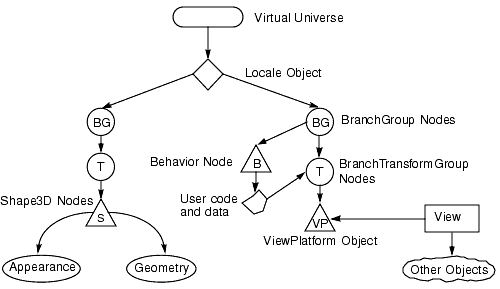
\includegraphics[width=\textwidth]{figures/java3d-overview}
\caption{A simple scene graph with view control}
\label{fig:java3d-overview}
\end{figure}

Amazon\footnote{\url{http://amazon.com}}, one of the biggest book retailors in
the world, accounts 227 programming books containing the term
Java3D~\cite{amazon2014java3d}. This is an important factor to be taken into
consideration, since 3D Application Programming Interfaces (APIs) are usually
non trivial, given the complexity related to the subject.

The downside of adopting this framework is that Sun Microsystems abandoned it
just after its source code was donated, on February 2008, under the terms of the
GNU General Public
License\footnote{\url{http://www.gnu.org/licenses/gpl-2.0.html}}. However, in
2012, Julien
Gouesse\footnote{\url{http://gouessej.wordpress.com/2012/08/01/java-3d-est-de-retour-java-3d-is-back}}
ported the last release of Java3D to the Java Binding for the OpenGL API (JOGL)
version 2.0\footnote{\url{http://jogamp.org/jogl/www}}, a library designed to
provide better and faster hardware-supported 3D graphics to applications written
in Java.
Java3D performance problems remain, and its APIs are outdated (it has not
received a single update in six years); but it has several books dedicated to
it, not to mention the expressive amount of code examples available on the
Internet.
These were sufficient reasons to choose it as the plug-in's graphics engine
during the development phase.

By the time that this text was being written, a new version of Java, the eighth
one, has been released by Oracle Corporation
\footnote{\url{http://www.oracle.com/technetwork/java/javase/8-whats-new-2157071.html}}.
The relevant fact is that the new version of JavaFX that is shipped with the
latest JDK now includes 3D Graphics features such as shapes, camera, lights,
subscene, material, picking, and antialiasing. This release makes JavaFX a
strong candidate to substitute the old Java3D technology, which was used to
develop the prototype and the plug-in. Though, more time is necessary to confirm
if this technology will become the \textit{de facto} standard of 3D development
in Java.

\section{Hosting environment}\label{sec:ide-choice}

The task of choosing an Integrated Development Environment (IDE) to host the
CodeForest plug-in started with three candidates, currently the most popular
IDEs amongst developers~\cite{furmankiewicz2008eclipse}:
Eclipse~\cite{eclipse2014eclipse}, NetBeans~\cite{netbeans2014netbeans}, and
IntelliJ IDEA~\cite{jetbrains2014intellij}; all of them available on the
Internet.

The three following questions were prepared in advance to aid our search to find
the most adequate IDE to integrate with. They embody the aspects that are
considered most relevant to the decision process.
\begin{enumerate}
  \item Which IDE has the highest market share?
  \item Are all IDEs free (as in ``free speech'')?
  \item Which one of them has the largest body of documentation available?
\end{enumerate}

Although there is not a large body of research to corroborate it, Eclipse seems
to be the winner of the Java IDE Wars~\cite{geer2005eclipse}. A research
conducted in 2012 found that, of 1800 participants that took part in an online
survey, 70\% pointed Eclipse as their primary development environment, followed
by 28\% of IntelliJ IDEA users and 17\% of NetBeans
users~\cite{rebel2012productivity}.

When analyzed under the perspective of price, both Eclipse and NetBeans stands
apart from IntelliJ IDEA. Jetbrains offer two editions of its IDE: Community and
Ultimate. The Community Edition works only with Java Standard Edition and it
has no cost. The Ultimate Edition works with both Java Standard and
Enterprise Edition and it costs US\$ 199 for individuals and US\$
499 for companies and organizations\footnote{Obtained from
\url{http://www.jetbrains.com/idea/buy/index.jsp} on September 9th of
2014.}.
Both Eclipse and NetBeans are open source products, freely offered by the
Eclipse Foundation and Oracle Corporation, with no restrictions of use.

From the documentation perspective, Amazon has for sale 286 Eclipse related
titles~\cite{amazon2014eclipse}. NetBeans can be found on 136
books~\cite{amazon2014netbeans} while IntelliJ Idea is the subject of a total of
23 books~\cite{amazon2014intellij}. This method to find out which one has the
biggest body of documentation available falls short of scientific rigor but it
can provide us with a strong indicator of which IDE is most documented.

When we take into consideration the questions initially defined and their
answers, the Eclipse IDE stands out as the most adequate platform to host the
CodeForest plug-in. It is the \textit{de facto} standard amongst developers, it
is free and freely distributed, and---according to our criterion---it has the
largest body of documentation available. These points are responsible for making
Eclipse our IDE of choice. Sections \ref{sec:eclipse} and \ref{sec:osgi}
provides a brief explanation about Eclipse, its history, and the underlying
technology about its runtime environment, OSGi.

\section{Eclipse}\label{sec:eclipse}

Eclipse began in 1999 as an IBM Canada project, whose goal was to unify all of
its development environments on a single codebase. Many of IBM's development
tools were written in Smalltalk\footnote{Smalltalk is an object-oriented,
dynamically typed, reflective programming language designed and created in the 1970s at the
Learning Research Group (LRG) of Xerox PARC~\cite{myers1998brief}.}, which was
rapidly losing market share to languages like Java. IBM's VisualAge for Java
IDE, named ``Best Product of the Year'' by InfoWorld in
2001\footnote{\url{http://www-03.ibm.com/press/us/en/pressrelease/1799.wss}},
was written in Smalltalk. The problem is that, except for IBM and a few other
vendors, the language did not have significant adoption in the industry. Thus,
IBM tasked its Object Technology International (OTI) group with creating a
highly extensible IDE based in Java. The Eclipse Platform goal was to eclipse
its competitor, Microsoft's Visual Studio~\cite{clayberg2008eclipse}.

At first sight, Eclipse might look like a giant piece of software---the latest
release, codename Luna---is estimated to have 61 million lines of
code~\cite{taft2014luna}. Contrariwise, it is structured as a small kernel
containing a plug-in loader, surrounded by hundreds of plug-ins.

The fundamental concept about the Eclipse platform is that everything is a
plug-in, where each subsystem that is part of the Eclipse Platform is itself
structured as a set of plug-ins that implement some function. Eclipse Software
Development Kit (Figure~\ref{fig:eclipsesdk}) includes the basic platform plus
two major tools designed for plug-in development. One is the Java Development
Tools (JDT) which implement a full featured Java development environment. The
other is the Plug-in Developer Environment (PDE), responsible for adding
specialized tools to leverage the development of plug-ins and
extensions~\cite{brownwilson2011archoss, eclipse2014architecture,
danjou2005java}.

\begin{figure}[h!]
\centering
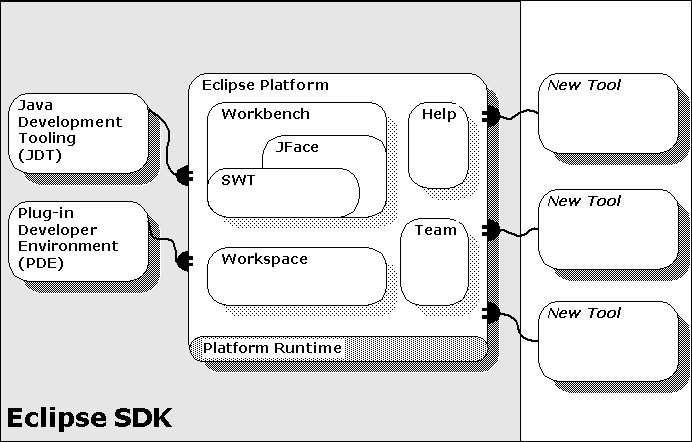
\includegraphics[width=.5\textwidth]{figures/sdk-arch}
\caption{Eclipse SDK architecture}
\label{fig:eclipsesdk}
\end{figure}

During the development of its third release, the Eclipse Foundation created a
sub-project called Equinox, aiming at replacing Eclipse's homegrown runtime platform
(called component model) with one that already existed, as well as
providing support for dynamic plug-ins. The team decided to implement the OSGi
(Section~\ref{sec:osgi}) specification as the underlying system in charge of
managing plug-ins. The rationale was to appeal to a broader community by
standardizing on a component model that had wider adoption outside the Eclipse
ecosystem~\cite{brownwilson2011archoss}. Migrating the original component model
to OSGi was the last major change made on Eclipse's
infrasctructure~\cite{blewitt2013eclipse}.

\section{OSGi}\label{sec:osgi}

Formerly known as the Open Services Gateway initiative (OSGi), the OSGi Alliance
was formed in March 1999 by a consortium of leading technology companies with
the mission to define a universal integration platform for the interoperability
of applications and services. OSGi provides a development platform based on
modular decoupled components and a pluggable dynamic service model for the Java
platform. A development platform, in the context of this research, is a set of
software libraries and tools that aid in the development of software components,
and the corresponding runtime environment that can host these developed
components.

\begin{figure}[h!]
\centering
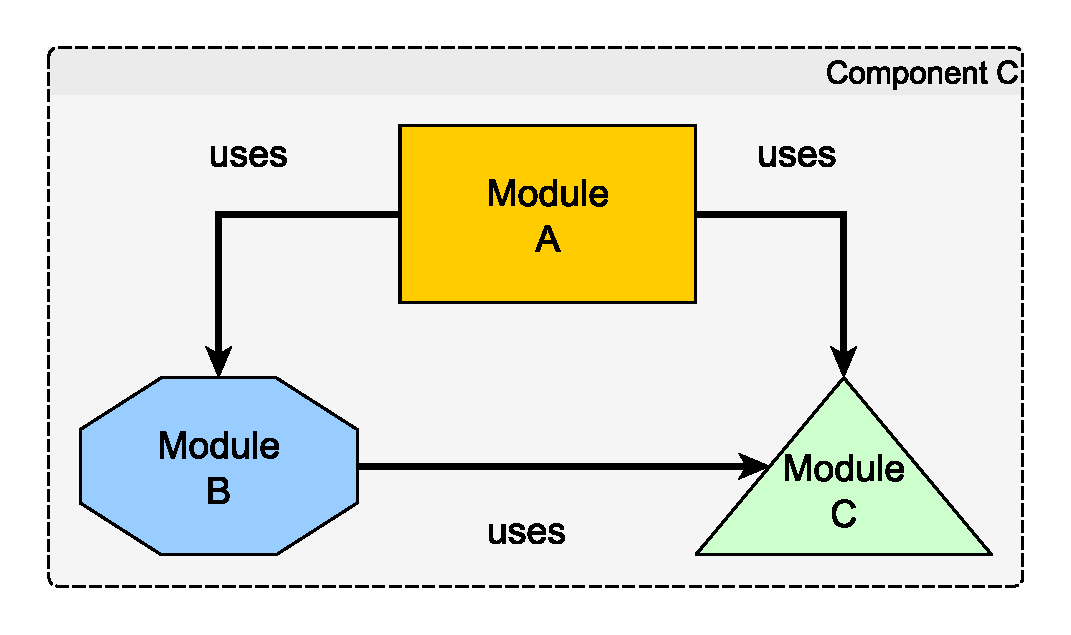
\includegraphics[width=.5\textwidth]{figures/modularity.eps}
\caption{A component decomposed into modules}
\label{fig:modularity}
\end{figure}

OSGi was conceived to target the lack of advanced modularization support in
standalone Java VM environments. Modularity here refers to the logical
decomposition of a large system into smaller collaborating pieces
(Figure~\ref{fig:modularity}). Java provides some aspects of modularity in the
form of object orientation, though Sun Microsystems did not make any plans to
add support for programming~\cite{hall2011osgi, castroalves2011osgi}.
There are plans to add a modular system to the Java VM and, according to the
most recent schedule, it will be available in Java
9\footnote{\url{http://openjdk.java.net/projects/jigsaw/}}. Meanwhile,
the resources available to developers are the language's standard mechanisms:
visibility modifiers---public, protected, private, and package private---and packages,
usually employed for purposes of partitioning code. Both of them solve low-level
object-oriented encapsulation issues~\cite{gosling2005java}. However, neither of
them are suited for logical system partitioning.

Another modularity issue present in the Java platform is the classpath; it
generally inhibits good modularity practices. The classpath is a location, a
place where the compiler will look for classes that the running application
demands to be loaded during runtime. In general, an application depends on
various versions of libraries and components. The classpath does not offer a way
to declare which code version a given application relies on; it returns the
first version found. As a result, large applications that depend on different
source code versions of the same library will probably fail at some point of
their lifetime. These kind of failures happen during runtime, from causes such
as NoSuchMethodError (when a wrong version of the class is loaded) or
ClassNotFoundException (when a wrong version of the library is loaded).

The OSGi framework is divided into three layers: module, lifecycle and service.
The \textbf{module layer} defines the OSGi module concept (called
\textit{bundle}). A bundle is a JAR file, with its own class loader, that
contains extra metadata which allow the developer to explicitly select packages
that are going to be visible to other packages. This mechanism extends the
access modifiers (public, private, and protected) provided by the language. The
\textbf{lifecycle layer} administers the application, supplying controls to
safely add and remove bundles without the need to restart the application.
Additionally, this layer lets components to be ``lazy loaded''; in other words,
a component is loaded by the application only when
required~\cite{brownwilson2011archoss}. Finally, the \textbf{services layer}
provides a way to publish services into a registry, while clients search the
registry to find available services to use. Services can appear and disappear at
any time~\cite{hall2011osgi, castroalves2011osgi}.

The flexibility, advanced controls of managed resources, and lifecycle control
offered by the OSGi framework make it the perfect foundation for the Eclipse
environment, whose main purpose is to be highly extensible, stable, and consume
minimum computational resources.

\section{Dependencies}\label{sec:dependencies}

To complete this research in a reasonable time, certain tradeoffs had to be
made, specially when it comes to transparently integrate the plug-in with other
tools developed by the members of the Software Analysis \& Experimentation Group
(SAEG).

One of such a tools is the Integration Coverage-based Debugging (ICD) tool
~\cite{souza13adding, souza2012depuracao}. ICD tool receives as input the MCP
and block coverages (Section~\ref{sec:bg-codecoverage}) of the test suite, the
chosen heuristic and the outcome of the tests (success or fail). It outputs the
MCP and block lists and the roadmap.
The input is generated by Instrumentation Strategies Simulator
(InSS)~\cite{souza2012depuracao}, which instruments the source code, executes
unit tests, and gathers the coverage data and the outcome of every test run.
Figure~\ref{fig:icd} describes how the InSS and ICD tools work together to
produce the guidelines for fault localization based on integration coverage.

The result of this process is outputted as an XML file, containing a set of
tuples. Each element of this set is a pair of (1) an element of the source code
(node, method, or class) that was exercised by unit tests and (2) a
suspiciousness score, assigned based on the results of applied heuristics.

\begin{figure}[h!]
\centering
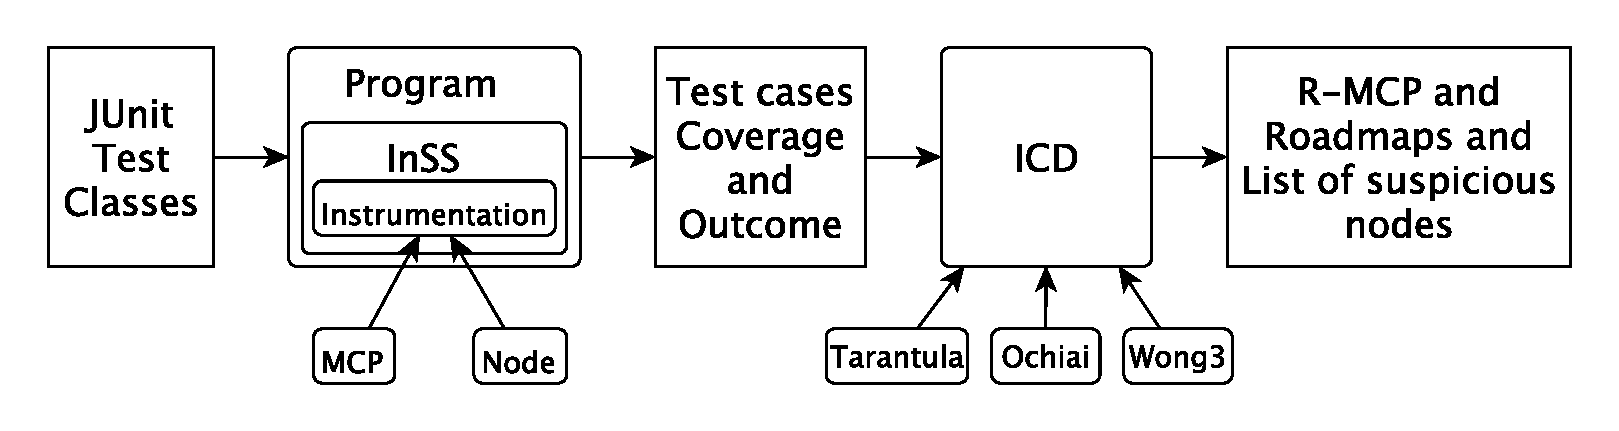
\includegraphics[width=\textwidth]{figures/icd_implementation}
\caption{ICD implementation}
\label{fig:icd}
\end{figure}

The current development state of the plug-in requires the execution in advance
of the ICD/InSS workflow and that the generated file be copied into the
project's root folder as ``codeforest.xml''. It is our intent to make these steps
transparent to the user in the future, absorbing them as a part of the plug-in's
functionality. It is expected that this feature would shorten feedback cycles of
the bug-fixing activity (Figure~\ref{fig:feedback-cycle}).

\begin{figure}[h!] \centering
\centerline{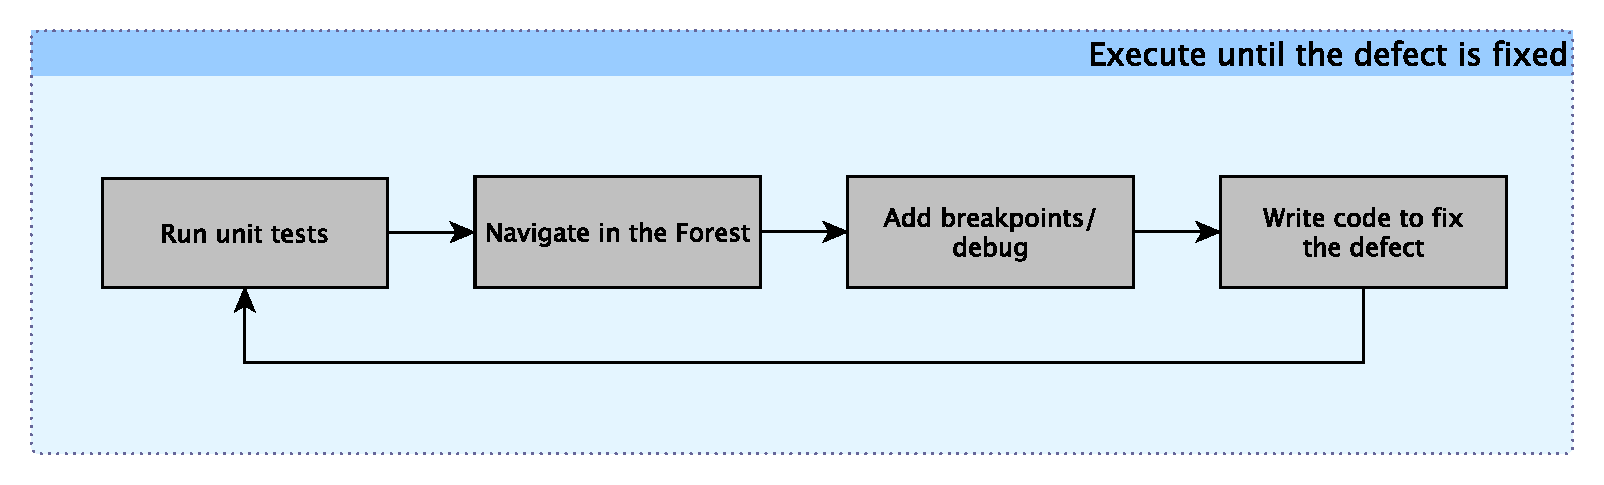
\includegraphics[width=\linewidth]{figures/feedback-loop}}
\caption{Bug-fixing feedback cycle}\label{fig:feedback-cycle}
\end{figure}

\section{Plug-in operation}

As previously explained, the plug-in is activated by the presence of a file
generated by the InSS tool~\cite{souza2012depuracao}, named ``codeforest.xml''
and located at the project's root directory (Figure~\ref{fig:operation-00}).
When this file is present, the developer that is operating the Eclipse IDE can
right-click the project under analysis.

\begin{figure}[h!]
\centerline{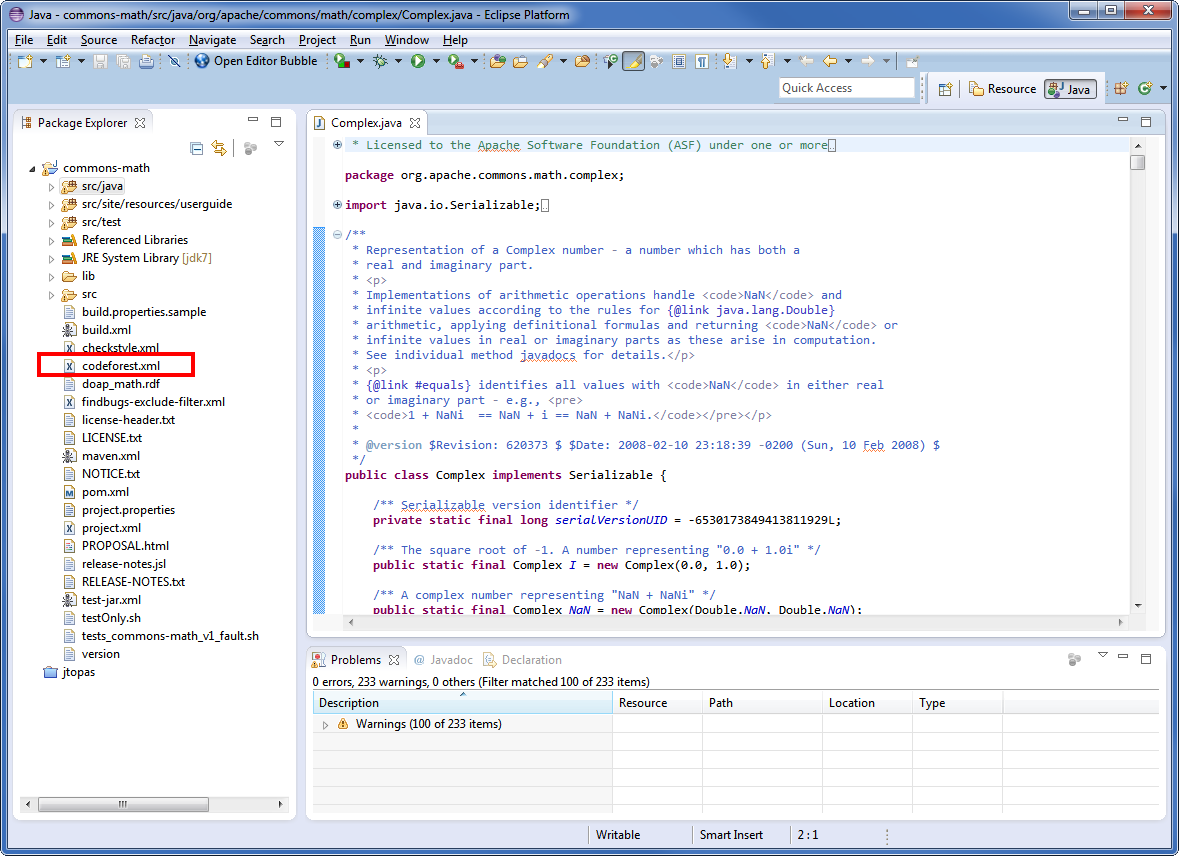
\includegraphics[width=.8\linewidth]{figures/commons_math_complex_00}}
\caption{A codeforest.xml file of Apache Commons Math
project}\label{fig:operation-00}
\end{figure}

When this action is fired, a popup menu is displayed; amongst its several
options, the CodeForest submenu is shown. At this point, the developer could
ignore the execution and continue his/her task at hand or select the ``Perform
analysis'' option (Figure~\ref{fig:operation-01}).

\begin{figure}[h!]
\centerline{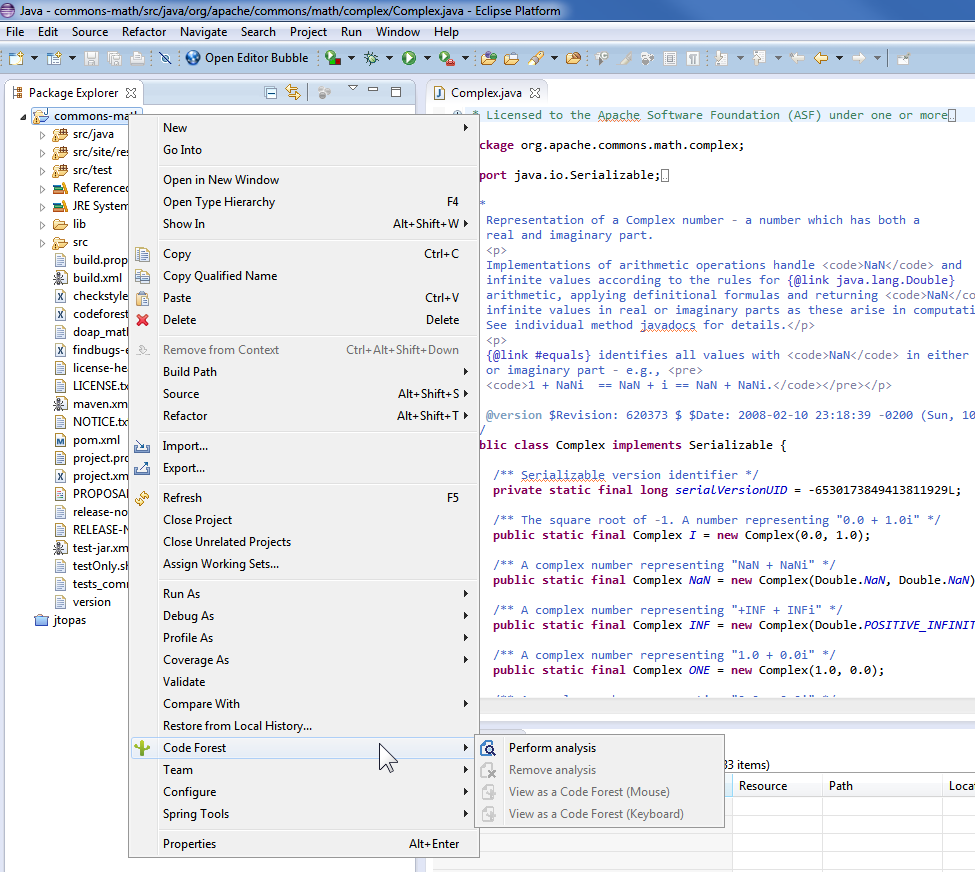
\includegraphics[width=.8\linewidth]{figures/commons_math_complex_01_perf_analysis}}
\caption{The CodeForest menu expanded}\label{fig:operation-01}
\end{figure}

A single left-click on the ``Perform analysis'' command runs a series of tasks,
whose output is that every Java file opened for edition is decorated, i.e., its
statements are painted according to suspiciousness values read from the XML file
(Figure~\ref{fig:operation-02}).
Internally, the plug-in parses the Java source code, identifies statements and
searches for its related data obtained from the input file (``codeforest.xml''). This architecture
enables the plug-in to display different data using the same infrastructure; it
only requires new adapters to read the data source and adapt it to the internal
domain objects.

\begin{figure}[h!]
\centerline{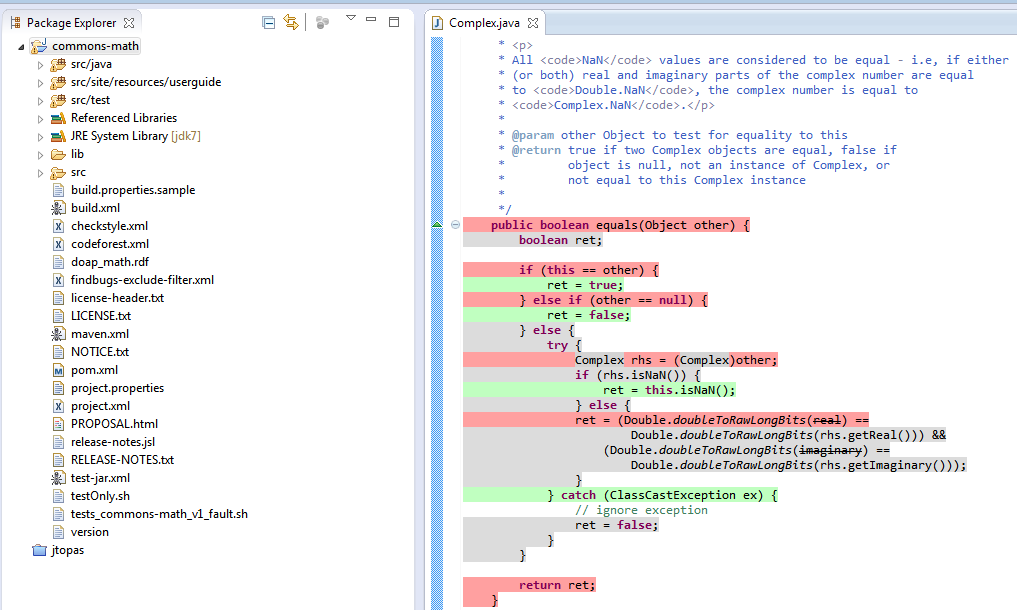
\includegraphics[width=.8\linewidth]{figures/commons_math_complex_02_red_green_grey}}
\caption{A method highlighted by the plug-in}\label{fig:operation-02}
\end{figure}

From this point onwards, the developer can keep the highlight
hints to aid debugging the system and/or navigate the codebase using the
CodeForest features (Figure~\ref{fig:operation-03}).

\begin{figure}[ht]
\centerline{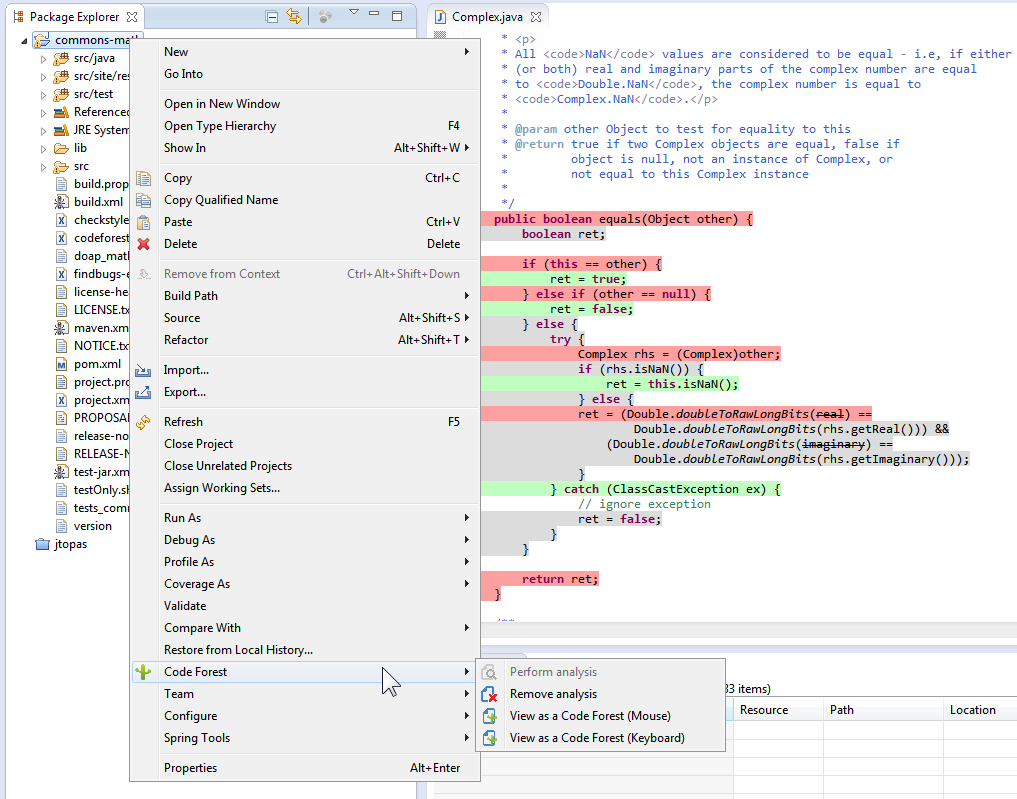
\includegraphics[width=.8\linewidth]{figures/commons_math_complex_03_open_view}}
\caption{Menu options after performing project analysis}\label{fig:operation-03}
\end{figure}

Choosing to display the CodeForest instructs the plug-in to open a smaller
version of it, still embedded inside the Eclipse IDE
(Figure~\ref{fig:operation-04}). From our observations during experiments with
the tool (Chapter~\ref{ch:cfexperimentation}), the recommended way to explore
the CodeForest is to detach it and drag the window into a separate screen.
Setting up the debugging environment this way allows the developer to freely
explore the forest, while keeping the source code visible all time, and
vice-versa.

\begin{figure}[ht]
\centerline{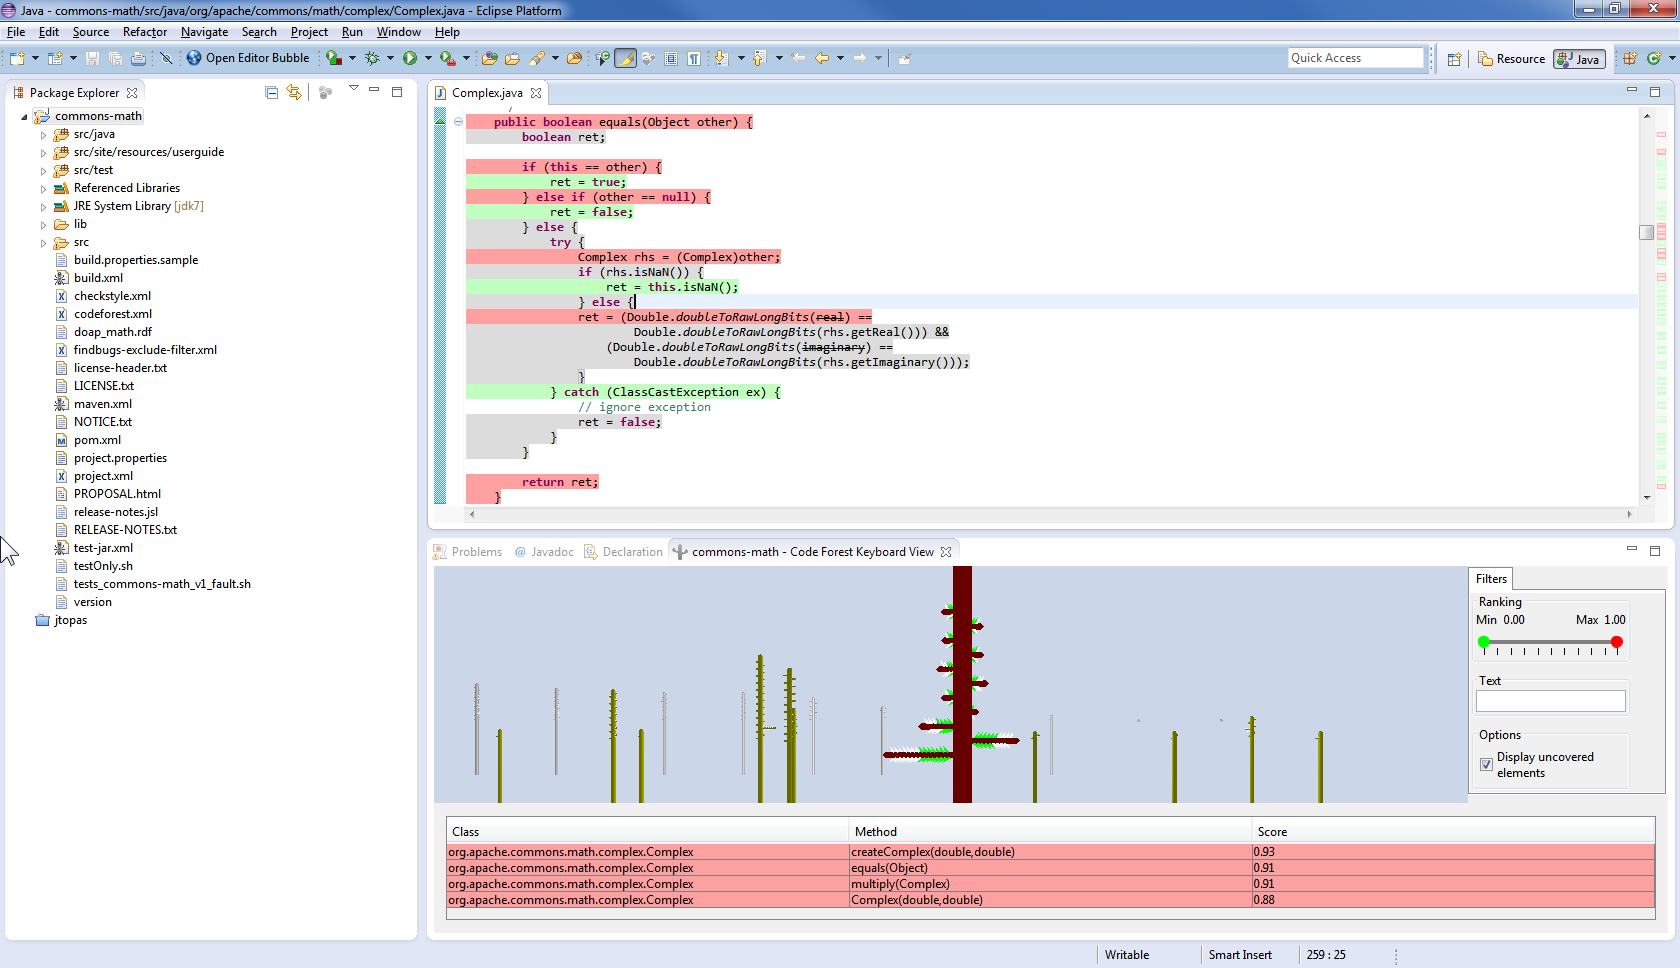
\includegraphics[width=.8\linewidth]{figures/commons_math_complex_05_view_min}}
\caption{CodeForest embedded inside Eclipse IDE}\label{fig:operation-04}
\end{figure}

The tools present in the prototype (trimmer and filter) remained a part of the
plug-in, and their functions were preserved. The trimmer
(Figure~\ref{fig:operation-05}--Area 2) excludes elements from the scene whose
ranking is out of a delimited range: by moving two sliders, the developer
defines the inferior and superior limits. The filter
(Figure~\ref{fig:operation-05}--Area 3) is responsible for searching the
codebase, looking for elements that contain the inputted term. It was
implemented as a simple, case-insensitive, textual search. Every element  that
does not contain the queried term is excluded from the scene. If there is one
line of code in a whole class that contains that term, then the forest will be
reduced to a single cactus, with one single-thorned branch. Both tools can work
together or independently.

The third tool present in the plug-in is the roadmap
(Figure~\ref{fig:operation-05}--Area 4). It contains a sequence of steps
(methods) that the developer is advised to follow in order to find the defect.
Items are painted with the color related to its ranking (red, orange, yellow,
and green). The roadmap is comprised of a limited list, ordered in decrescent
order of suspiciousness, and is not a tool per se, but a kind of smart shortcut
to the other tools. When one of the items of the list is picked, both trimmer
and filter are parameterized with data from that element. The term to be
searched is the name of the method, excluded its signature---the method
``createComplex(double,double)'' sets up the query ``createComplex''. The
trimmer's range is delimited inferiorly by the method's suspiciousness score and
superiorly by the same score added of a 3\% delta~\cite{souza2012depuracao}.

Finally, there is the CodeForest (Figure~\ref{fig:operation-05}--Area 1), the
virtual environment that lets developers navigate through the codebase,
represented as a forest of cacti. The rationale behind the construction of the
forest is explained in details in Chapter~\ref{ch:forest}. The developer
interacts with elements using keyboard and mouse.

The keyboard is used to move the developer through the forest. Arrow keys move
the observer forward (up), backward (down), left (left), and right (right). In
this kind of basic movement, the observer always face forward. Modifier keys
change the nature of the movement. Alt key combined with one of the arrows makes
the observer move up or down, emulating the climbing or descending of a ladder.
Control (Windows and Linux) or Command (MacOS) key emulates the ``neck''
movement, making the observer thinks that his or her head is moving up, down,
turning left or right.

The developer uses the mouse in a ``point and click'' fashion. When in need of
opening the source code file associated with any desired element, he/she clicks
it with the mouse's left button. This action fires a task that opens a Java
Editor window containing the Java file related to that element, and positions
the cursor at the appropriate location---a click on a cactus will put the cursor
at the line where the class is declared; on a branch positions the cursor at the
method's declaration; a thorn will open at the corresponding line of code.

At any time, the developer can access the CodeForest menu by right-clicking the
project and selecting the ``Remove analysis'' option. This will close the
CodeForest window and remove the highlight of every file within the current
project.

\begin{figure}[h!]
\centerline{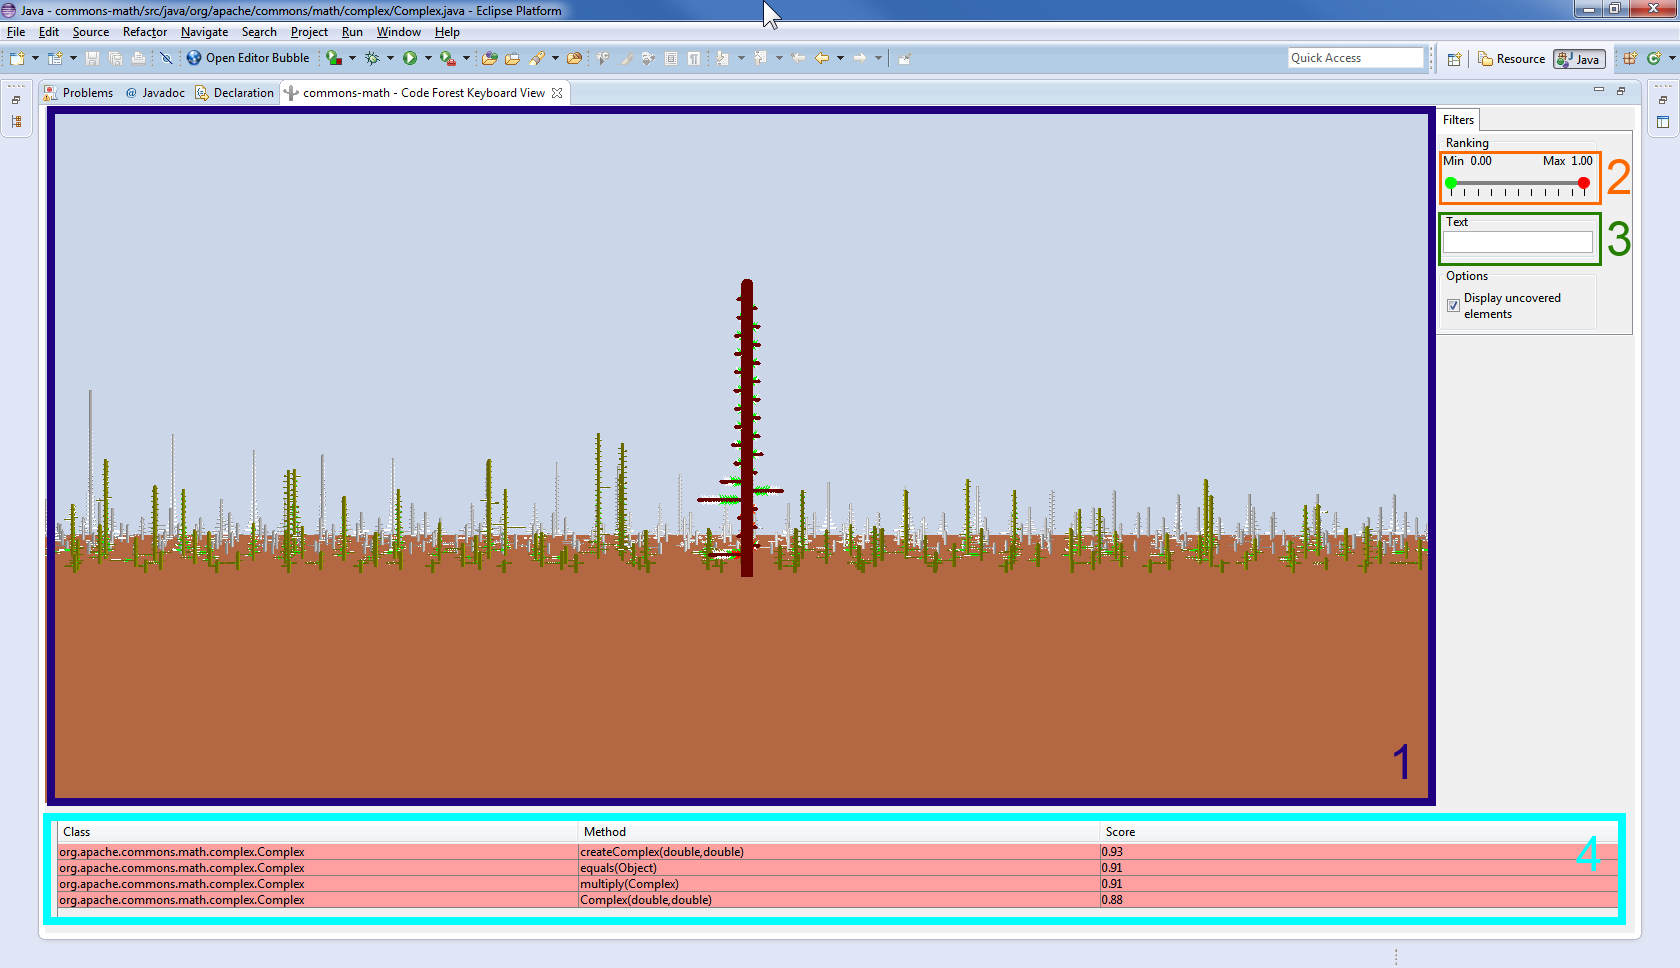
\includegraphics[width=\linewidth]{figures/commons_math_complex_04_view_max_numbers}}
\caption{Maximized view of CodeForest and its elements}\label{fig:operation-05}
\end{figure}

\section{Final remarks}

This chapter presented the architectural and technical forces that guided the
development of the CodeForest as a plug-in embedded on an Integrated Development
Environment (IDE). It also explained the external dependencies and how they
integrate with the plug-in. A brief explanation of the tools that are part of
the plug-in and how to utilize them was also given.

The following chapter describes the experiment that has been set up to evaluate
the plug-in. It points the opinions, insights and any other information gathered
that could guide future enhancements and adjustments in the tool.